\documentclass[titlepage]{jarticle}
\usepackage[dvipdfmx]{graphicx}
\usepackage{amsmath}
\usepackage{amssymb}
\usepackage{amsfonts}
\usepackage{comment}
\usepackage{listings}
\usepackage{here}
\usepackage{r04ec-exp}
\usepackage{cases}
%
\lstset{
  basicstyle={\ttfamily},
  identifierstyle={\small},
  commentstyle={\smallitshape},
  keywordstyle={\small\bfseries},
  ndkeywordstyle={\small},
  stringstyle={\small\ttfamily},
  frame={tb},
  breaklines=true,
  columns=[l]{fullflexible},
  numbers=left,
  xrightmargin=0zw,
  xleftmargin=3zw,
  numberstyle={\scriptsize},
  stepnumber=1,
  numbersep=1zw,
  lineskip=-0.5ex,
  language=c
}
\renewcommand{\lstlistingname}{ソースコード}
\makeatletter
\newcommand{\figcaption}[1]{\def\@captype{figure}\caption{#1}}
\newcommand{\tblcaption}[1]{\def\@captype{table}\caption{#1}}
\makeatother
%%% 表紙の記載事項設定
%
% 実験題目  ※レポートを書くときは,まず,タイトルを正しいものに変えましょう
%
\title{フーリエ解析-前半}
% 学年・番号
\grade{4年37番}%
% 氏名
\author{本間 三暉}
% 班(後期は班に分かれて実験をする.そのときは,ここに班番号を記入する.)
\team{}
% 提出日
\date{2023年1月30日}
% 実験日
\expdate{2023年1月5日,1月19日,1月31日,2月9日}
% 共同実験者
% グループに分かれて実験をするテーマでは,グループメンバーの番号名前を書く.
\coauthor{%
2番 & 飯吉 可南子\\
17番 & 酒井 優花\\
23番 & 関 玖祥\\
28番 & 中村 洋介\\
33番 & 羽田 伊吹\\
35番 & 福田 啓悟
}
%
%記載例:
%\coauthor{%
%  2番 & 新潟 花子\\
%  11番 & 三条 次郎}
%%
\begin{document}
\maketitle
\section{研究テーマ}
声色の解析による発言の信憑性の確認

\section{背景・目的}
\subsection{背景}
警察ではよくポリグラフ検査という嘘をついているかどうかを見る検査が取り調べで行われる.
しかし,これは取り調べられている人が不整脈等の病気でない必要がある.
よって,取り調べられている人の健康状態によらない検査を確立する必要がある.

\subsection{目的}
声の高さや話すスピードと嘘の相関関係を明らかにする.

\section{DFTの理論}
\begin{eqnarray}
  f(t) &=& \frac{b_0}{2} + \sum_{n = 1}^{\infty}\{b_n\cos(n\omega_0 t)+a_n\sin(n\omega_0 t)\} \label{equ:1} \\
  f(t) &=& \sum_{n=-\infty}^\infty c_n e^{in\omega_0t} \label{equ:3}
\end{eqnarray}
\begin{numcases}
  {\int^{\tau + T}_{\tau}e^{i(n-m)\omega_0t}dt =}
  0 \ (n \neq m) & \nonumber \\
  T \ (n = m) & \label{equ:4}
\end{numcases}
\begin{eqnarray}
  c_m&=&\frac{1}{T}\int_\tau^{\tau+T}f(t)e^{-im\omega_0t}dt \label{equ:5} \\
  X_l&=&\sum_{k=0}^{N-1}x_k(W_N)^{kl}\Delta t \label{equ:16}
\end{eqnarray}

\subsection{Q1 式\ref{equ:1}中の基本振動, 5倍振動を表す項を書き出せ.}
基本振動項: $b_1\cos(\omega_0t)+a_1\sin(\omega_0t)$

5倍振動項: $b_5\cos(5\omega_0t)+a_5\sin(5\omega_0t)$

\subsection{Q2 式\ref{equ:1}中の移動項の時間平均はいくらか.また,$\displaystyle\frac{b_0}{2}$の値の意味を答えよ.}
振動項は周期関数であるので, 時間平均は0.
$\displaystyle\frac{b_0}{2}$は$f(t)$の時間平均.

\subsection{Q3 式\ref{equ:1}に含まれる$n$倍振動項の振幅と, それを$\cos(\omega_0t)$と比較した時の位相のずれを求めよ.}
$n$倍振動項: $b_n\cos(n\omega_0t)+a_n\sin(n\omega_0t)$

これを$\sin$に合成すると,
$\displaystyle\sqrt{a_n^2+b_n^2}\cos\left(n\omega_0t - \arctan\frac{a_n}{b_n}\right)$
が得られる.
よって,

振幅: $\sqrt{a_n^2+b_n^2}$

位相のずれ: $\displaystyle\arctan\frac{a_n}{b_n}$

\subsection{Q4 式\ref{equ:1}から式\ref{equ:3}に書き換える場合, 係数$c_n$はどのように決められるか. $a_n, b_n$との関係式を答えよ.}
$e^{\pm in\omega_0t}=\cos(n\omega_0t)\pm i\sin(n\omega_0t)$より,

\begin{eqnarray}
  \cos(n\omega_0t) &=& \frac{e^{in\omega_0t} + e^{-in\omega_0t}}{2} \nonumber \\
  \sin(n\omega_0t) &=& \frac{e^{in\omega_0t} - e^{-in\omega_0t}}{2i} \nonumber
\end{eqnarray}

となる.
式\ref{equ:1}に代入して,

\begin{equation*}
  f(t) = \displaystyle\frac{b_0}{2} + \frac{1}{2}\sum_{n = 1}^{\infty}\{(b_n-ia_n)e^{in\omega_0t}+(b_n+ia_n)e^{-in\omega_0t}\}
\end{equation*}

を得る. これを式\ref{equ:3}と比較して,

\begin{numcases}
  {c_n=}
  \frac{b_n - ia_n}{2} \ (n > 0) & \nonumber \\
  \frac{b_0}{2} \ (n = 0) & \nonumber \\
  \frac{b_n + ia_n}{2} \ (n < 0) & \nonumber
\end{numcases}

\subsection{Q5 式\ref{equ:3}の中で, 3倍振動を表す項を書き出せ.}
$c_3e^{i3\omega_0t}+c_{-3}e^{-i3\omega_0t}$

\subsection{Q6 $c_n$と$c_{-n}$の関係を答えよ. ただし, $f(t)$は実関数とする.}
$c_n$と$c_{-n}$は互いに共役である.

\subsection{Q7 $n$倍振動項($n>0$)について考える. 複素数$c_n$を極形式で,
$c_n=|c_n|e^{i\delta_n}$
のように書いたとする.
絶対値$|c_n|$と偏角$\delta_n$は, 何を表しているか. (Q3と比較せよ)}

$c_ne^{in\omega_0t}=|c_n|e^{i(n\omega_0t+\delta_n)}$となり,
これをQ3と比較する.
式\ref{equ:1}と\ref{equ:3}の$n$の範囲の違いを考慮すると$|c_n|$は$n$倍振動の振幅の半分,
$\delta_n$は位相のずれを表していることがわかる.

\subsection{Q8 式\ref{equ:4}が成り立つことを確かめよ.}
$n \neq m$のとき,

\begin{eqnarray}
  \int_\tau^{\tau+T}e^{i(n-m)\omega_0t}dt&=&\frac{1}{i(n-m)\omega_0}\left[e^{i(n-m)\omega_0t}\right]_\tau^{\tau+T}\nonumber\\
  &=&\frac{e^{i(n-m)\omega_0\tau}}{i(n-m)\omega_0}\left(e^{i(n-m)\omega_0T}-1\right)\nonumber\\
  &=&0\nonumber
\end{eqnarray}

$n=m$のとき, $n-m=0$なので,

\begin{equation*}
  \int_\tau^{\tau+T}e^{i(n-m)\omega_0t}dt=\int_\tau^{\tau+T}dt=T
\end{equation*}

\subsection{Q9 式\ref{equ:5}が成り立つことを確かめよ.}
式\ref{equ:4}より,
\begin{equation*}
  \frac{1}{T}\int_\tau^{\tau+T}f(t)e^{-im\omega_0t}dt
  = \frac{1}{T}\sum^\infty_{n=-\infty}\int^{\tau+T}_{\tau}c_ne^{i(n-m)\omega_0t}dt
  = \frac{1}{T}c_mT=c_m
\end{equation*}

\subsection{Q10 フーリエ成分$X(\omega)$は何を意味しているのだろうか.}
$f(t)$のうち, 角周波数が$\omega$の成分の振幅を表している.

\subsection{Q11 式\ref{equ:16}から, $X_l=X_{l+N}$を示せ.}
\begin{equation*}
  X_{l+N}=\sum_{k=0}^{N-1}x_k(W_N)^{k(l+N)}\Delta t
  =\sum_{k=0}^{N-1}x_k(W_N)^{kl}\Delta t(W_N)^{kN}
\end{equation*}

ここで,
$(W_N)^{KN}=\left(e^{-i\frac{2\pi}{N}}\right)^{KN}=e^{-i2\pi k}=1$
なので,

\begin{equation*}
  X_{l+N}=\sum_{k=0}^{N-1}x_k(W_N)^{kl}\Delta t=X_l
\end{equation*}

\subsection{Q12 $X_l=X_{l+N}$ということは,
フーリエ成分$X_l$と$X_{l+N}$とが区別できないことを示している.
これは, 扱うデータが離散的だからである. この事情を図を用いて説明せよ.}

$\sin t$上から等間隔で値を取った6点と$\sin t$, $\sin(6t)$を重ねたグラフを図\ref{fig:12}
に示す.

\begin{figure}[H]
  \centering
  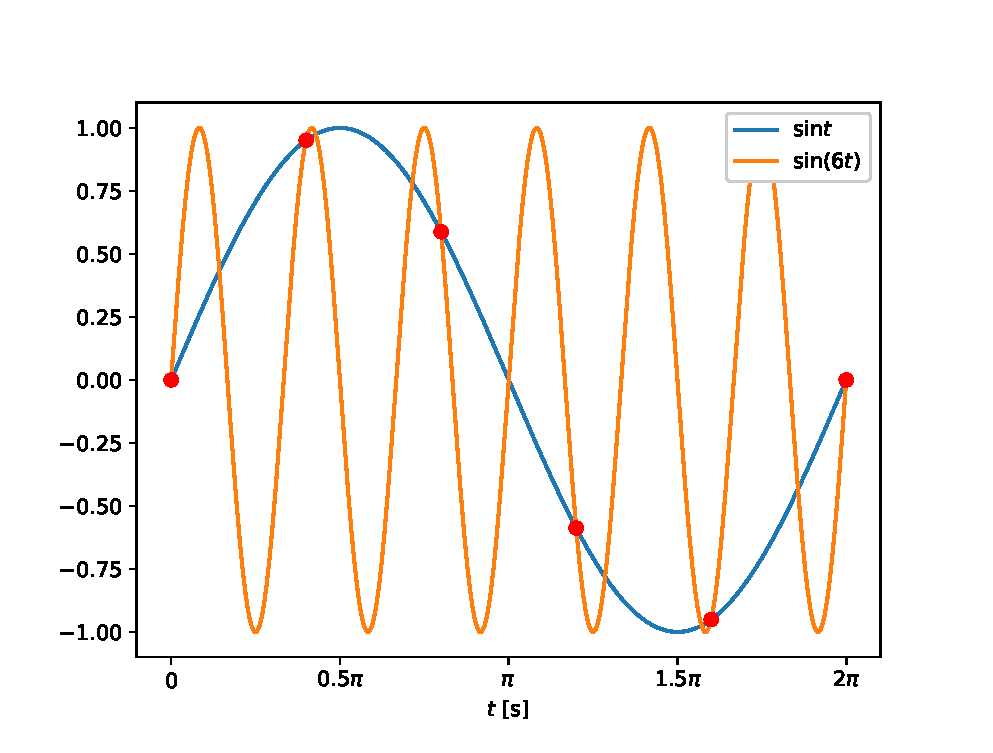
\includegraphics[width=0.6\hsize]{img/12.eps}
  \caption{}
  \label{fig:12}
\end{figure}

図を見ると,
抽出点だけを見たときにそれが$\sin t$を表しているのか$\sin(6t)$を表しているのか
区別ができないことがわかる.

\subsection{Q13 $X_{N-2}$と$X_2$の間にはどんな関係があるか.}
\begin{eqnarray}
  X_{2}&=&\sum_{k=0}^{N-1}x_k(W_N)^{2k}\Delta t\nonumber\\
  X_{N-2}&=&\sum_{k=0}^{N-1}x_k(W_N)^{N-2}\Delta t\nonumber\\
  &=&\sum_{k=0}^{N-1}x_k(W_N)^{-2k}\Delta t(W_N)^{kN}\nonumber
\end{eqnarray}

$(W_N)^{kN}=1$より,

\begin{equation*}
  X_{N-2}=\sum_{k=0}^{N-1}x_k(W_N)^{-2k}\Delta t
\end{equation*}

$W_N=e^{-i\frac{2\pi}{N}}$なので,
$X_{N-2}$と$X_2$は共役にある.

\subsection{Q14 フーリエ成分$\{X_l\}$から, 元の信号列$\{x_k\}$を再現するための式を作れ.}
\begin{eqnarray}
  X_l &=& \sum^{N - 1}_{k = 0}x_k(W_N)^{kl}\Delta t \nonumber \\
  \leftrightarrow \sum^{N - 1}_{l = 0}X_l(W_N)^{-kl} &=& \sum^{N - 1}_{l = 0}\sum^{N - 1}_{k = 0}x_k(W_N)^{k(l - l)}\Delta t \nonumber
\end{eqnarray}

式\ref{equ:4}より, $\displaystyle\sum^{N - 1}_{k = 0}(W_N)^{k(l-l)}=N$であるので,
これを上の式に代入すると,

\begin{eqnarray}
  \sum^{N - 1}_{l = 0}X_l(W_N)^{-kl} &=& x_kN\Delta t \nonumber \\
  \leftrightarrow x_k &=& \frac{1}{N\Delta t}\sum^{N - 1}_{l = 0}X_l(W_N)^{-kl} \nonumber
\end{eqnarray}

\section{自作プログラムの仕様・動作例}

\subsection{プログラムの仕様}
DFTの理論を元に作成したDFTプログラムの主要部をソースコード\ref{dft.c}に示す.
\begin{lstlisting}[caption=DFT,label=dft.c]
for (int k = 0; k < n; k++) {
  real[k] = 0;
  imag[k] = 0;
  for (int j = 0; j < n; j++) {
    real[k] += amp[j] * cos(2 * M_PI * k * j / n)*dt;
    imag[k] += amp[j] * sin(2 * M_PI * k * j / n)*dt;
  }
  amplitude[k] = sqrt(real[k] * real[k] + imag[k] * imag[k]);
}
\end{lstlisting}
このあとでamplitudeを表示すれば良い.

\subsection{動作例}
$sin( 2 \pi t)+sin(100 \times 2 \pi t)$を入力信号としてDFTを通したものを図\ref{1_100}に示す.
\begin{figure}[H]
  \centering
  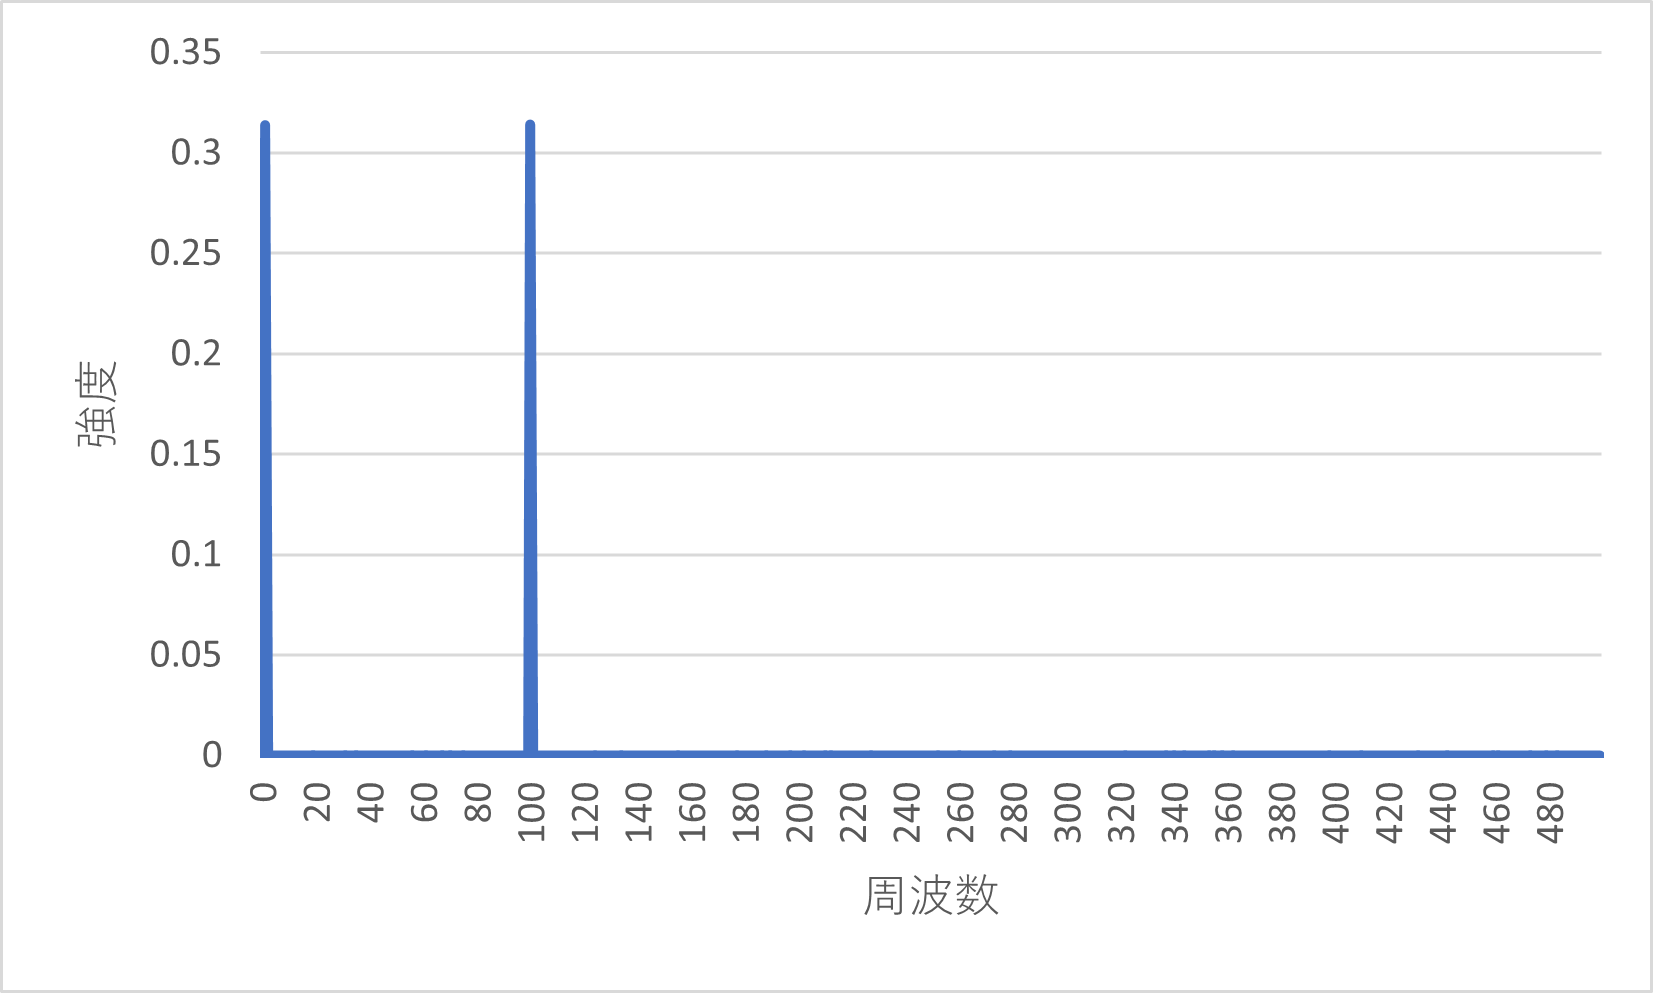
\includegraphics[width=0.6\hsize]{img/1_100.png}
  \caption{$sin(2 \pi t)+sin(100 \times 2 \pi t)$を入力信号として与えた場合}
  \label{1_100}
\end{figure}

$sin(100 \times 2 \pi t)$の係数を20にした$sin(2 \pi t)+20sin(100 \times 2 \pi t)$を入力信号としてDFTを通したものを図\ref{1_20-100}に示す.
\begin{figure}[H]
  \centering
  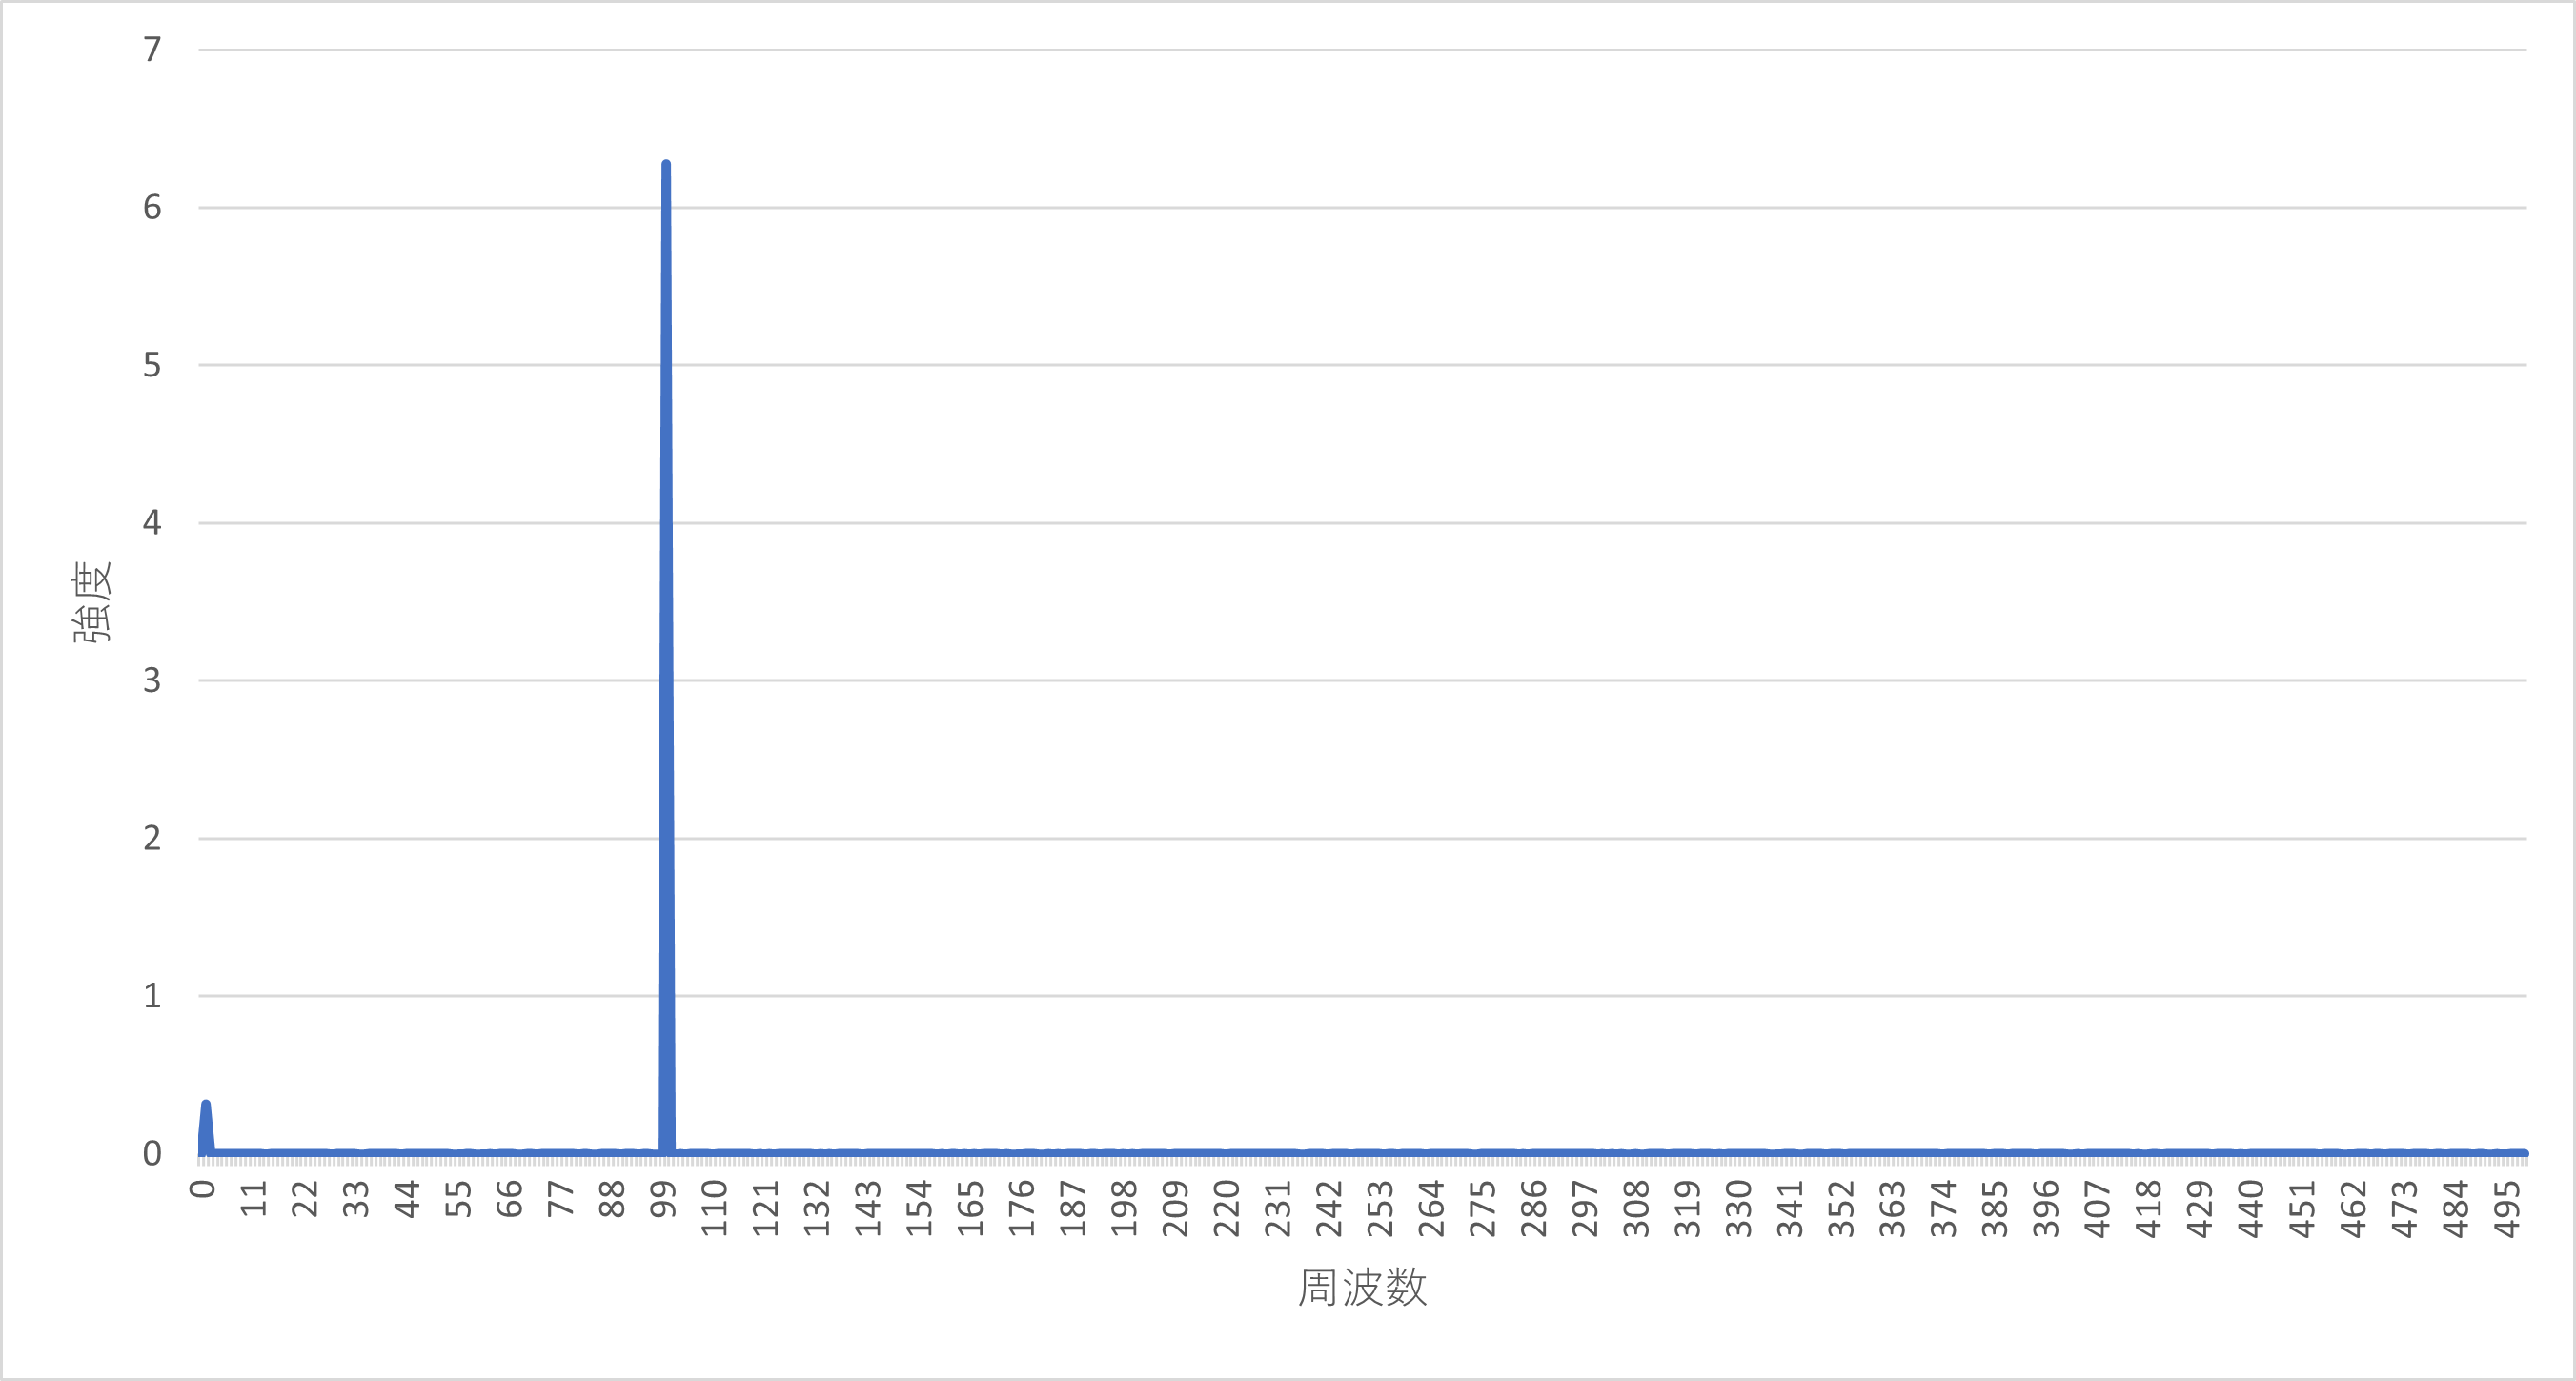
\includegraphics[width=0.6\hsize]{img/1_20-100.png}
  \caption{$sin( 2 \pi t)+20sin(100 \times 2 \pi t)$を入力信号として与えた場合}
  \label{1_20-100}
\end{figure}
以上の結果からDFTのアルゴリズムは問題ないことがわかる.

\section{使用機材}
\begin{itemize}
  \item マイク
\end{itemize}

\section{実験方法・手順}
\begin{enumerate}
  \item 制御4年の学生数名に「はい」か「いいえ」で答えられる問に全て
        「いいえ」と答えてもらい,それを録音する.質問は次の通りとする.
        \begin{enumerate}
          \item あなたは長岡高専の学生ですか(嘘)
          \item あなたは電気電子システム工学科の学生ですか(本当)
          \item あなたは現在4年生ですか(嘘)
          \item あなたは雪を見た事がありませんね?(本当)
        \end{enumerate}
  \item 録音した音声の長さを記録する.この長さを話すスピードの評価値とする
  \item フーリエ解析により周波数解析を行う.
  \item それぞれの問に対する返答に周波数と音声の長さという2値のパラメータにおいて
        比較し,どのような違いがあるか評価する.
\end{enumerate}

\section{結果}
共同実験者6人に上で示した4つの質問を行った結果を図\ref{ibuki1}から\ref{yuuka4}に示す.
\begin{figure}[H]
  \begin{minipage}{0.495\hsize}
    \centering
    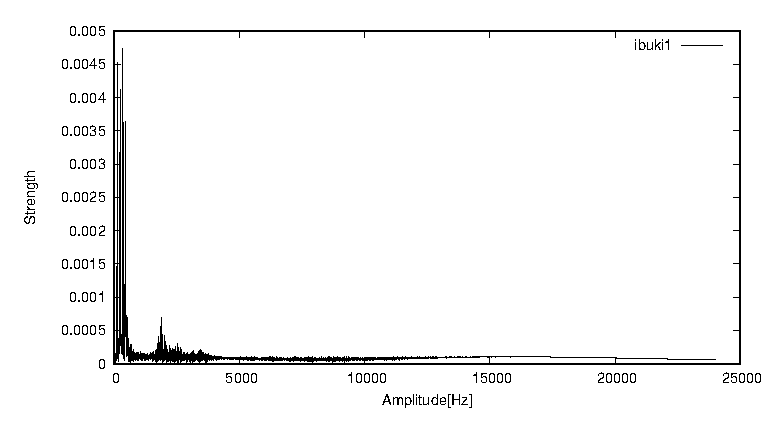
\includegraphics[width=8cm]{img/ibuki1.eps}
    \caption{羽田\_(a)}
    \label{ibuki1}
  \end{minipage}
  \begin{minipage}{0.495\hsize}
    \centering
    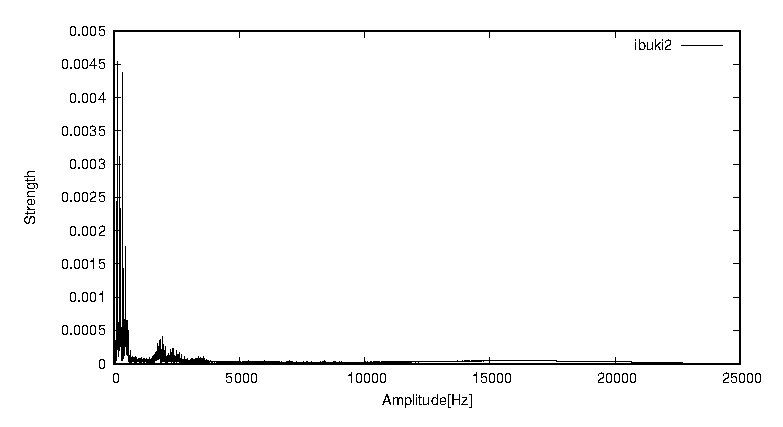
\includegraphics[width=8cm]{img/ibuki2.eps}
    \caption{羽田\_(b)}
    \label{ibuki2}
  \end{minipage}

  \begin{minipage}{0.495\hsize}
    \centering
    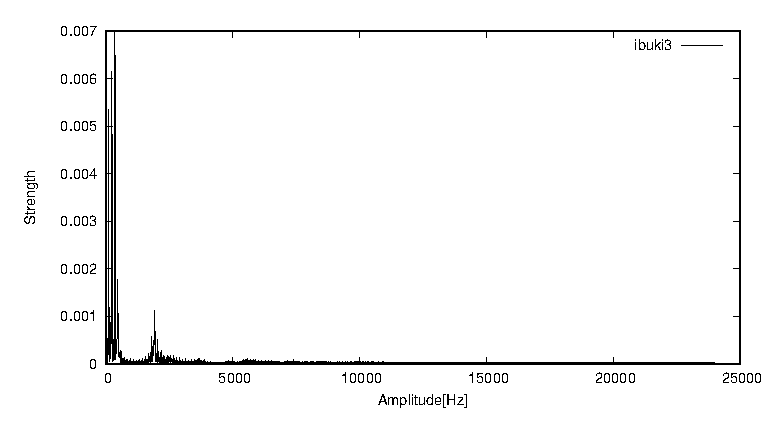
\includegraphics[width=8cm]{img/ibuki3.eps}
    \caption{羽田\_(c)}
    \label{ibuki3}
  \end{minipage}
  \begin{minipage}{0.495\hsize}
    \centering
    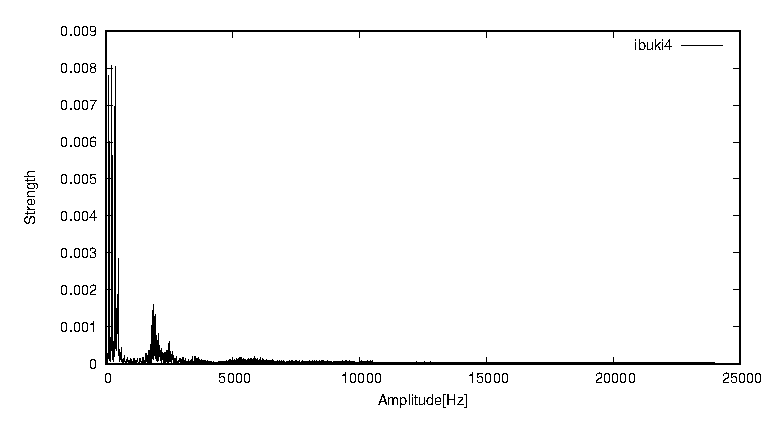
\includegraphics[width=8cm]{img/ibuki4.eps}
    \caption{羽田\_(d)}
    \label{ibuki4}
  \end{minipage}
\end{figure}

\begin{figure}[H]
  \begin{minipage}{0.495\hsize}
    \centering
    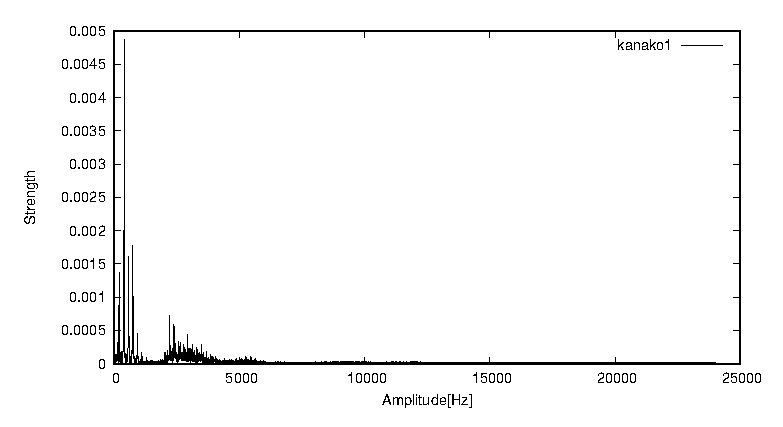
\includegraphics[width=8cm]{img/kanako1.eps}
    \caption{飯吉\_(a)}
    \label{kanako1}
  \end{minipage}
  \begin{minipage}{0.495\hsize}
    \centering
    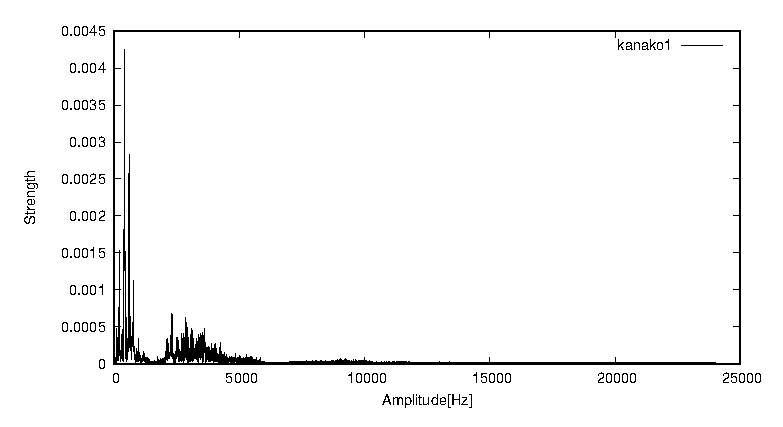
\includegraphics[width=8cm]{img/kanako2.eps}
    \caption{飯吉\_(b)}
    \label{kanako2}
  \end{minipage}

  \begin{minipage}{0.495\hsize}
    \centering
    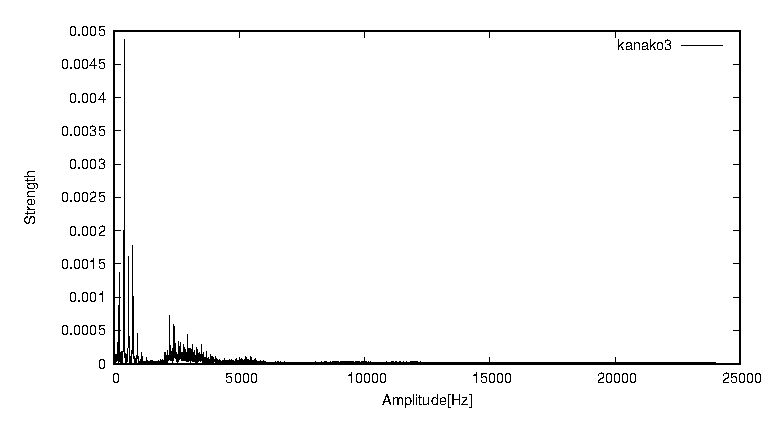
\includegraphics[width=8cm]{img/kanako3.eps}
    \caption{飯吉\_(c)}
    \label{kanako3}
  \end{minipage}
  \begin{minipage}{0.495\hsize}
    \centering
    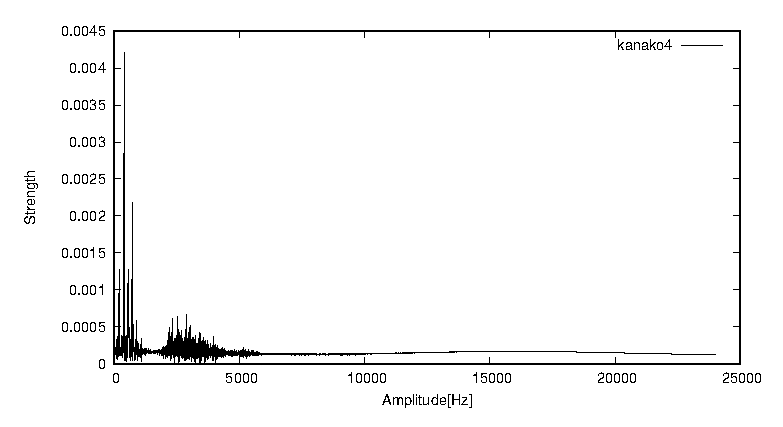
\includegraphics[width=8cm]{img/kanako4.eps}
    \caption{飯吉\_(d)}
    \label{kanako4}
  \end{minipage}
\end{figure}

\begin{figure}[H]
  \begin{minipage}{0.495\hsize}
    \centering
    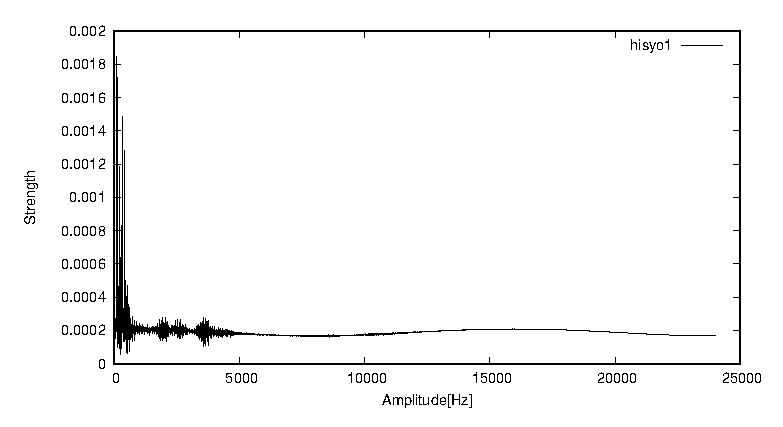
\includegraphics[width=8cm]{img/hisyo1.eps}
    \caption{関\_(a)}
    \label{hisyo1}
  \end{minipage}
  \begin{minipage}{0.495\hsize}
    \centering
    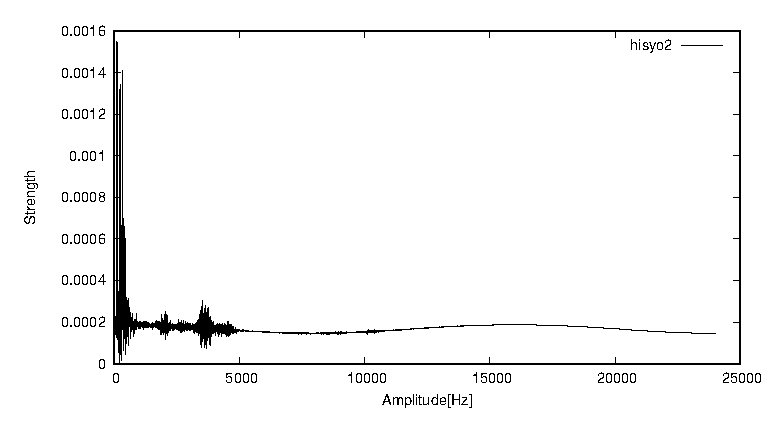
\includegraphics[width=8cm]{img/hisyo2.eps}
    \caption{関\_(b)}
    \label{hisyo2}
  \end{minipage}


  \begin{minipage}{0.495\hsize}
    \centering
    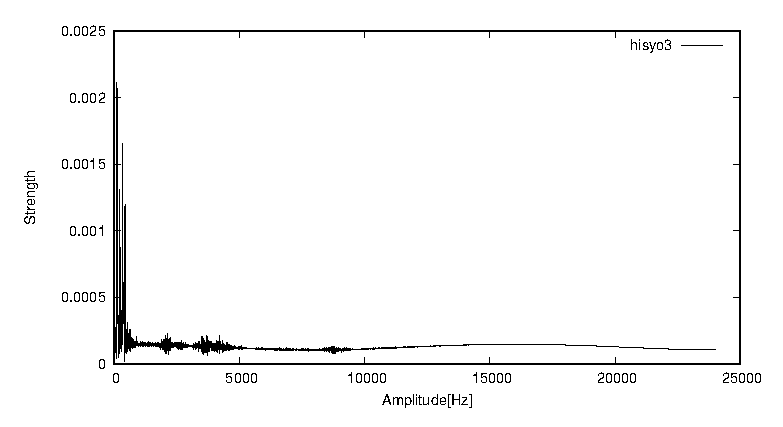
\includegraphics[width=8cm]{img/hisyo3.eps}
    \caption{関\_(c)}
    \label{hisyo3}
  \end{minipage}
  \begin{minipage}{0.495\hsize}
    \centering
    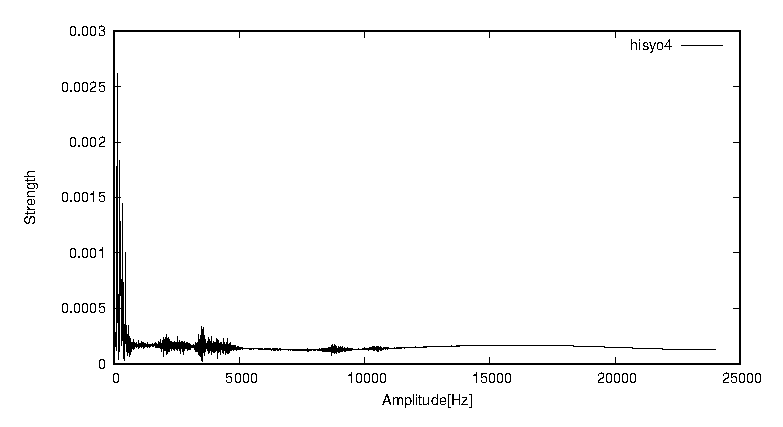
\includegraphics[width=8cm]{img/hisyo4.eps}
    \caption{関\_(d)}
    \label{hisyo4}
  \end{minipage}
\end{figure}

\begin{figure}[H]
  \begin{minipage}{0.495\hsize}
    \centering
    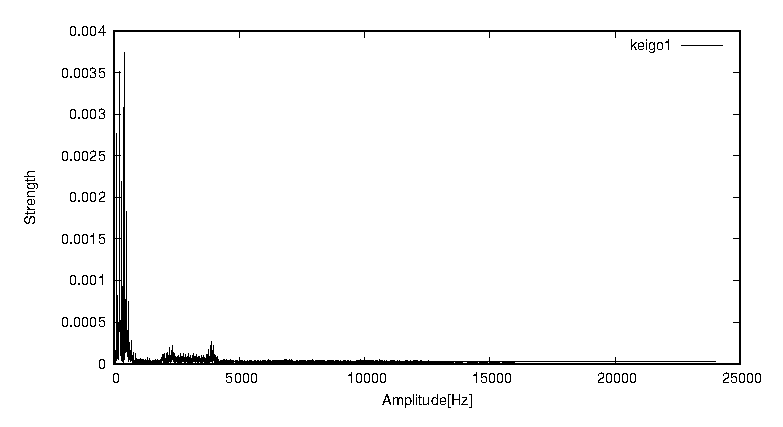
\includegraphics[width=8cm]{img/keigo1.eps}
    \caption{福田\_(a)}
    \label{keigo1}
  \end{minipage}
  \begin{minipage}{0.495\hsize}
    \centering
    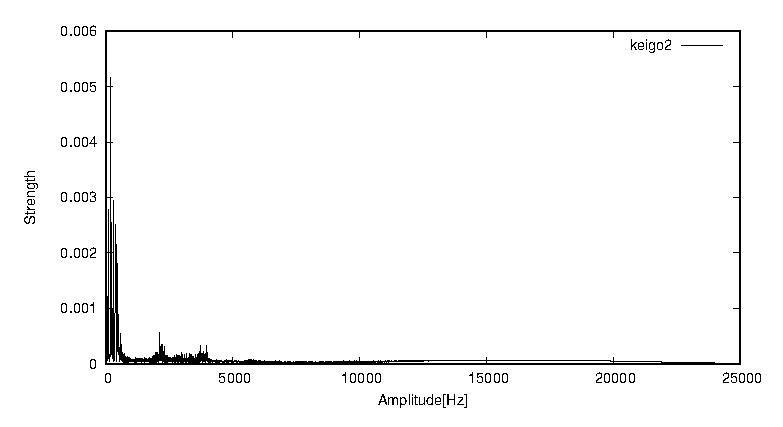
\includegraphics[width=8cm]{img/keigo2.eps}
    \caption{福田\_(b)}
    \label{keigo2}
  \end{minipage}


  \begin{minipage}{0.495\hsize}
    \centering
    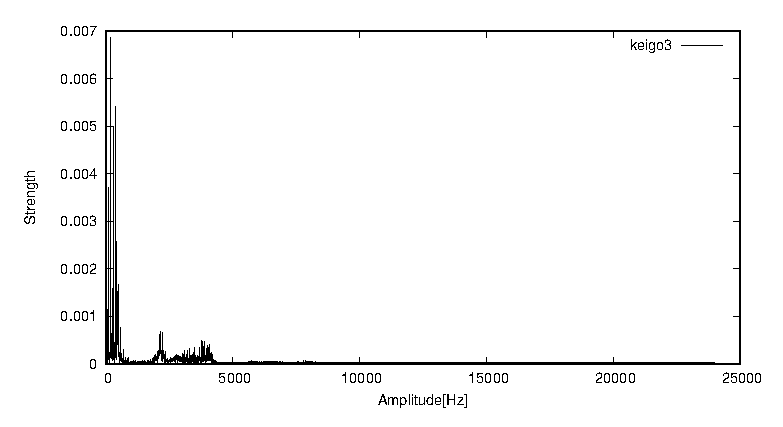
\includegraphics[width=8cm]{img/keigo3.eps}
    \caption{福田\_(c)}
    \label{keigo3}
  \end{minipage}
  \begin{minipage}{0.495\hsize}
    \centering
    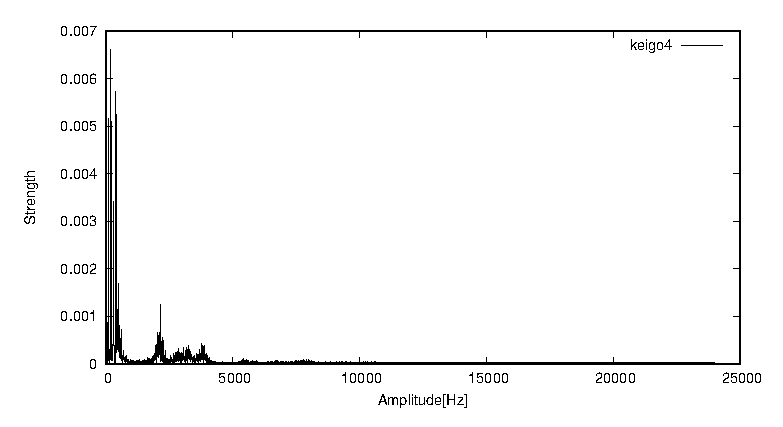
\includegraphics[width=8cm]{img/keigo4.eps}
    \caption{福田\_(d)}
    \label{keigo4}
  \end{minipage}
\end{figure}

\begin{figure}[H]
  \begin{minipage}{0.495\hsize}
    \centering
    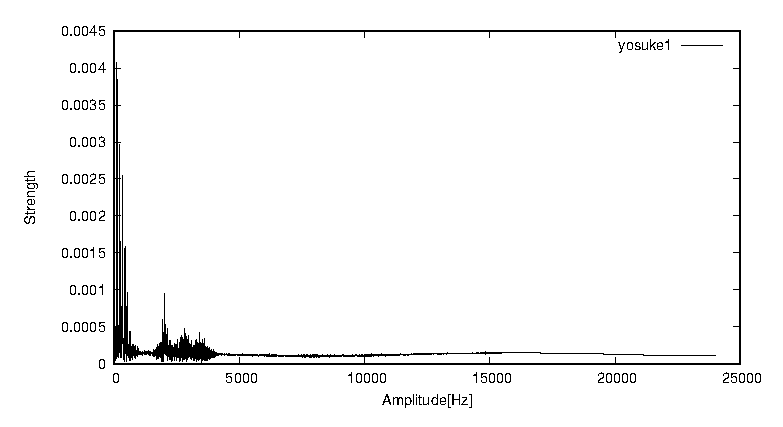
\includegraphics[width=8cm]{img/yosuke1.eps}
    \caption{中村\_(a)}
    \label{yosuke1}
  \end{minipage}
  \begin{minipage}{0.495\hsize}
    \centering
    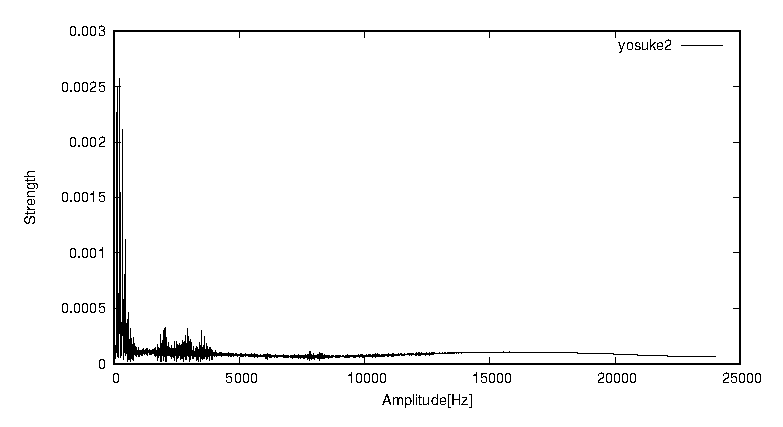
\includegraphics[width=8cm]{img/yosuke2.eps}
    \caption{中村\_(b)}
    \label{yosuke2}
  \end{minipage}


  \begin{minipage}{0.495\hsize}
    \centering
    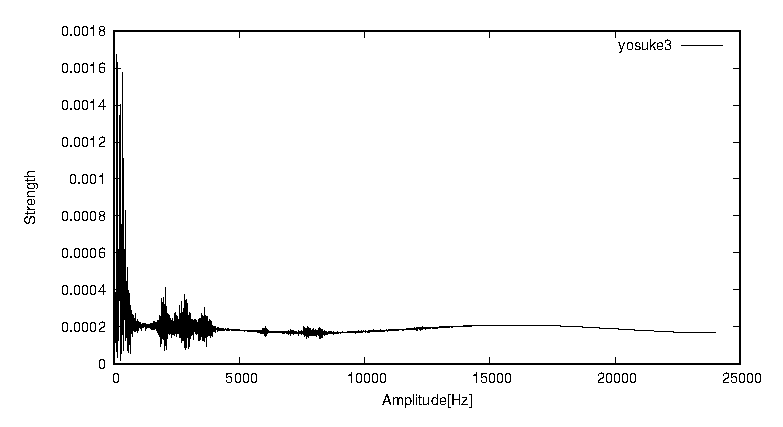
\includegraphics[width=8cm]{img/yosuke3.eps}
    \caption{中村\_(c)}
    \label{yosuke3}
  \end{minipage}
  \begin{minipage}{0.495\hsize}
    \centering
    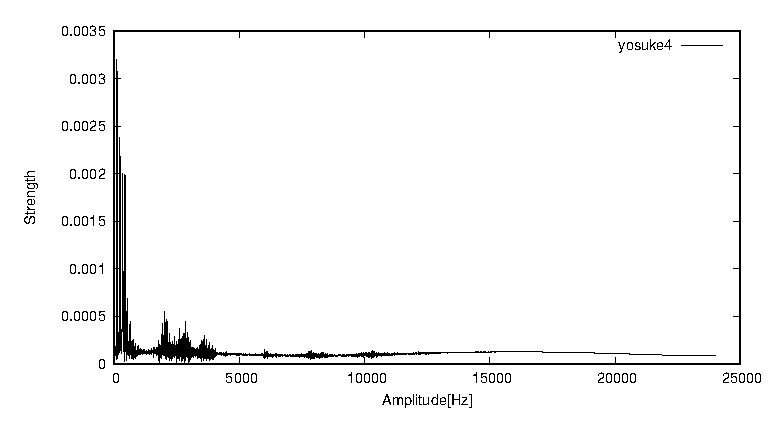
\includegraphics[width=8cm]{img/yosuke4.eps}
    \caption{中村\_(d)}
    \label{yosuke4}
  \end{minipage}
\end{figure}

\begin{figure}[H]
  \begin{minipage}{0.495\hsize}
    \centering
    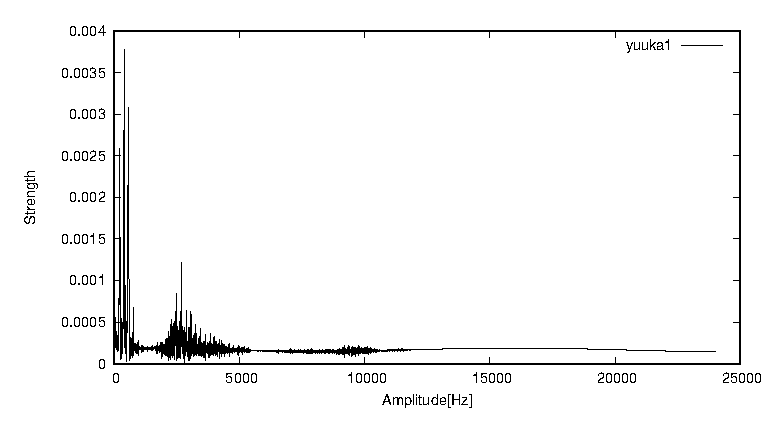
\includegraphics[width=8cm]{img/yuuka1.eps}
    \caption{酒井\_(a)}
    \label{yuuka1}
  \end{minipage}
  \begin{minipage}{0.495\hsize}
    \centering
    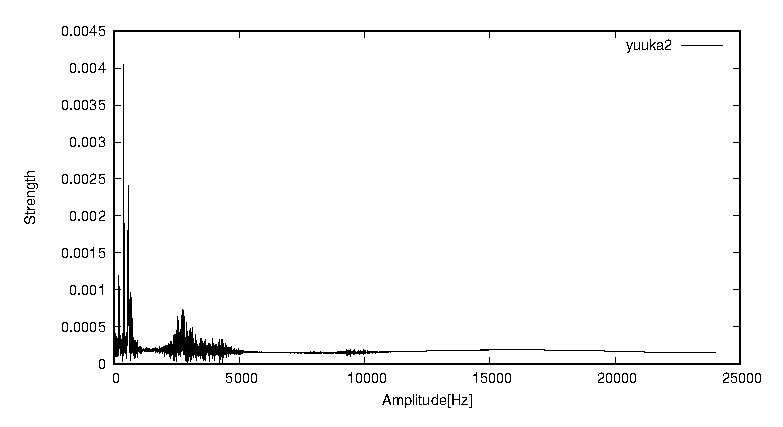
\includegraphics[width=8cm]{img/yuuka2.eps}
    \caption{酒井\_(b)}
    \label{yuuka2}
  \end{minipage}


  \begin{minipage}{0.495\hsize}
    \centering
    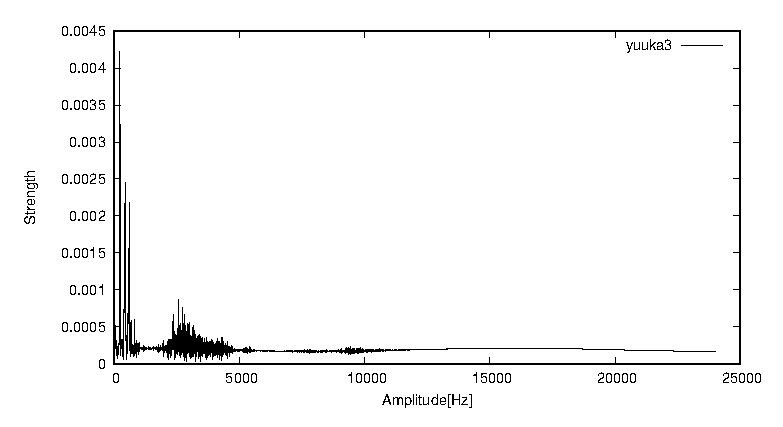
\includegraphics[width=8cm]{img/yuuka3.eps}
    \caption{酒井\_(c)}
    \label{yuuka3}
  \end{minipage}
  \begin{minipage}{0.495\hsize}
    \centering
    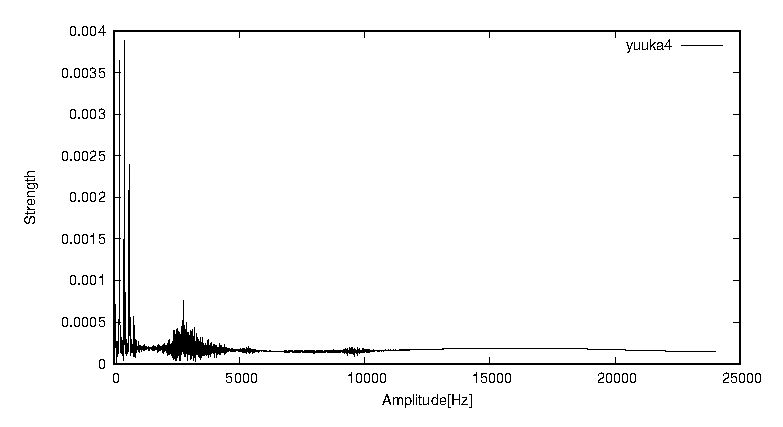
\includegraphics[width=8cm]{img/yuuka4.eps}
    \caption{酒井\_(d)}
    \label{yuuka4}
  \end{minipage}
\end{figure}

縦軸に話すスピードとしてサンプル数,横軸に強度が一番強い周波数を取ったものをまとめたものを図\ref{result}に示す.
\begin{figure}[H]
  \centering
  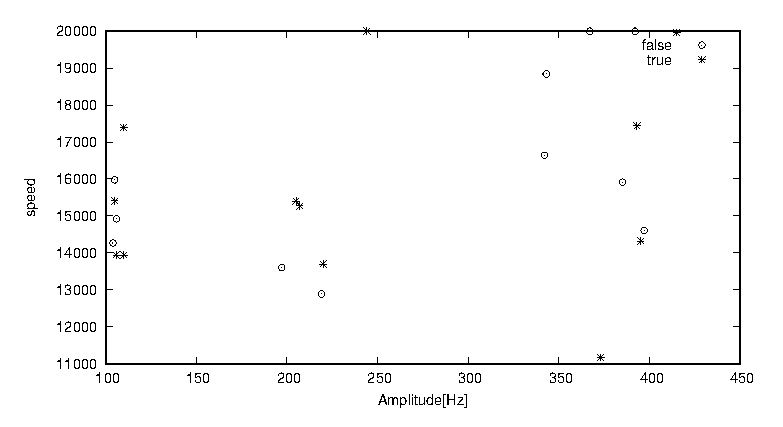
\includegraphics[width=14cm]{img/result.eps}
  \caption{話すスピードと強度の強い周波数の関係}
  \label{result}
\end{figure}

\section{考察}
今回は強度が最も強かった周波数と話すスピードについてまとめてみた.
しかし,これといった規則性を見つけることはできなかった.

このような結果になった原因として,
6人に対して質問が4つでは全体的にサンプル数が足りなかったことや,
比較するパラメータが間違っていたり足りなかった可能性があること,
強度が最も強い周波数には嘘による影響が出ない可能性があること,
質問に対する返答が作業になってしまい嘘をついているという状態ではなかった可能性があること
などが挙げられる.

\section{感想}
今回計画から実験まで自分で行ってみて,計画性の甘さや詰めの甘さなどが目立った.
来年の卒業研究では計画的に進め質の高い研究ができるように頑張りたい.

\section*{参考文献}
\begin{enumerate}
  \item 令和4年度電子制御工学実験 $\cdot$ 4年後期テキスト
\end{enumerate}
\end{document}